\documentclass[10pt,ignorenonframetext,compress, aspectratio=169]{beamer}
\setbeamertemplate{caption}[numbered]
\setbeamertemplate{caption label separator}{: }
\setbeamercolor{caption name}{fg=normal text.fg}
\beamertemplatenavigationsymbolsempty
\usepackage{lmodern}
\usepackage{amssymb,amsmath,mathtools}
\usepackage{ifxetex,ifluatex}
\usepackage{fixltx2e} % provides \textsubscript
\ifnum 0\ifxetex 1\fi\ifluatex 1\fi=0 % if pdftex
  \usepackage[T1]{fontenc}
  \usepackage[utf8]{inputenc}
\else % if luatex or xelatex
  \ifxetex
    \usepackage{mathspec}
  \else
    \usepackage{fontspec}
  \fi
  %%\defaultfontfeatures{Ligatures=TeX,Scale=MatchLowercase}
  \defaultfontfeatures{Scale=MatchLowercase}
\fi
\usetheme[]{metropolis}
% use upquote if available, for straight quotes in verbatim environments
\IfFileExists{upquote.sty}{\usepackage{upquote}}{}
% use microtype if available
\IfFileExists{microtype.sty}{%
\usepackage{microtype}
\UseMicrotypeSet[protrusion]{basicmath} % disable protrusion for tt fonts
}{}
\newif\ifbibliography
\usepackage{color}
\usepackage{fancyvrb}
\newcommand{\VerbBar}{|}
\newcommand{\VERB}{\Verb[commandchars=\\\{\}]}
\DefineVerbatimEnvironment{Highlighting}{Verbatim}{commandchars=\\\{\}}
% Add ',fontsize=\small' for more characters per line
\usepackage{framed}
\definecolor{shadecolor}{RGB}{248,248,248}
\newenvironment{Shaded}{\begin{snugshade}}{\end{snugshade}}
\newcommand{\KeywordTok}[1]{\textcolor[rgb]{0.13,0.29,0.53}{\textbf{{#1}}}}
\newcommand{\DataTypeTok}[1]{\textcolor[rgb]{0.13,0.29,0.53}{{#1}}}
\newcommand{\DecValTok}[1]{\textcolor[rgb]{0.00,0.00,0.81}{{#1}}}
\newcommand{\BaseNTok}[1]{\textcolor[rgb]{0.00,0.00,0.81}{{#1}}}
\newcommand{\FloatTok}[1]{\textcolor[rgb]{0.00,0.00,0.81}{{#1}}}
\newcommand{\ConstantTok}[1]{\textcolor[rgb]{0.00,0.00,0.00}{{#1}}}
\newcommand{\CharTok}[1]{\textcolor[rgb]{0.31,0.60,0.02}{{#1}}}
\newcommand{\SpecialCharTok}[1]{\textcolor[rgb]{0.00,0.00,0.00}{{#1}}}
\newcommand{\StringTok}[1]{\textcolor[rgb]{0.31,0.60,0.02}{{#1}}}
\newcommand{\VerbatimStringTok}[1]{\textcolor[rgb]{0.31,0.60,0.02}{{#1}}}
\newcommand{\SpecialStringTok}[1]{\textcolor[rgb]{0.31,0.60,0.02}{{#1}}}
\newcommand{\ImportTok}[1]{{#1}}
\newcommand{\CommentTok}[1]{\textcolor[rgb]{0.56,0.35,0.01}{\textit{{#1}}}}
\newcommand{\DocumentationTok}[1]{\textcolor[rgb]{0.56,0.35,0.01}{\textbf{\textit{{#1}}}}}
\newcommand{\AnnotationTok}[1]{\textcolor[rgb]{0.56,0.35,0.01}{\textbf{\textit{{#1}}}}}
\newcommand{\CommentVarTok}[1]{\textcolor[rgb]{0.56,0.35,0.01}{\textbf{\textit{{#1}}}}}
\newcommand{\OtherTok}[1]{\textcolor[rgb]{0.56,0.35,0.01}{{#1}}}
\newcommand{\FunctionTok}[1]{\textcolor[rgb]{0.00,0.00,0.00}{{#1}}}
\newcommand{\VariableTok}[1]{\textcolor[rgb]{0.00,0.00,0.00}{{#1}}}
\newcommand{\ControlFlowTok}[1]{\textcolor[rgb]{0.13,0.29,0.53}{\textbf{{#1}}}}
\newcommand{\OperatorTok}[1]{\textcolor[rgb]{0.81,0.36,0.00}{\textbf{{#1}}}}
\newcommand{\BuiltInTok}[1]{{#1}}
\newcommand{\ExtensionTok}[1]{{#1}}
\newcommand{\PreprocessorTok}[1]{\textcolor[rgb]{0.56,0.35,0.01}{\textit{{#1}}}}
\newcommand{\AttributeTok}[1]{\textcolor[rgb]{0.77,0.63,0.00}{{#1}}}
\newcommand{\RegionMarkerTok}[1]{{#1}}
\newcommand{\InformationTok}[1]{\textcolor[rgb]{0.56,0.35,0.01}{\textbf{\textit{{#1}}}}}
\newcommand{\WarningTok}[1]{\textcolor[rgb]{0.56,0.35,0.01}{\textbf{\textit{{#1}}}}}
\newcommand{\AlertTok}[1]{\textcolor[rgb]{0.94,0.16,0.16}{{#1}}}
\newcommand{\ErrorTok}[1]{\textcolor[rgb]{0.64,0.00,0.00}{\textbf{{#1}}}}
\newcommand{\NormalTok}[1]{{#1}}
\usepackage{longtable,booktabs}
\usepackage{caption}
% These lines are needed to make table captions work with longtable:
\makeatletter
\def\fnum@table{\tablename~\thetable}
\makeatother

% Prevent slide breaks in the middle of a paragraph:
\widowpenalties 1 10000
\raggedbottom

\AtBeginPart{
  \let\insertpartnumber\relax
  \let\partname\relax
  \frame{\partpage}
}
\AtBeginSection{
  \ifbibliography
  \else
    \let\insertsectionnumber\relax
    \let\sectionname\relax
    \frame{\sectionpage}
  \fi
}
\AtBeginSubsection{
  \let\insertsubsectionnumber\relax
  \let\subsectionname\relax
  \frame{\subsectionpage}
}

\setlength{\parindent}{0pt}
\setlength{\parskip}{6pt plus 2pt minus 1pt}
\setlength{\emergencystretch}{3em}  % prevent overfull lines
\providecommand{\tightlist}{%
  \setlength{\itemsep}{0pt}\setlength{\parskip}{0pt}}
\setcounter{secnumdepth}{0}

%% GLS Added
% Textcomp for various common symbols
\usepackage{textcomp}

\usepackage{booktabs}

% Creative Commons Icons
\usepackage[scale=1]{ccicons}

\newenvironment{centrefig}{\begin{figure}\centering}{\end{figure}}
\newcommand{\columnsbegin}{\begin{columns}}
\newcommand{\columnsend}{\end{columns}}
\newcommand{\centreFigBegin}{\begin{figure}\centering}
\newcommand{\centreFigEnd}{\end{figure}}
%%

\DefineVerbatimEnvironment{Highlighting}{Verbatim}{commandchars=\\\{\}, fontsize=\tiny}
% make console-output smaller:
\makeatletter
\def\verbatim{\tiny\@verbatim \frenchspacing\@vobeyspaces \@xverbatim}
\makeatother

%\setlength{\parskip}{0pt}

\setlength{\OuterFrameSep}{-4pt} % was -4pt
\makeatletter
\preto{\@verbatim}{\topsep=-10pt \partopsep=-10pt} % were 10pt
\makeatother

\title{Generalized Linear models}
\author{Gavin L. Simpson}
\date{February, 2017}

\begin{document}
\frame{\titlepage}

\section{Generalized linear models}\label{generalized-linear-models}

\begin{frame}{Generalized linear models}

\begin{itemize}
\tightlist
\item
  Generalised linear models (GLMs) are a synthesis and extension of
  linear regression plus Poisson, logistic and other regression models
\item
  GLMs extend the types of data and error distributions that can be
  modelled beyond the Gaussian data of linear regression
\item
  With GLMs we can model count data, binary/presence absence data, and
  concentration data where the response variable is not continuous.
\item
  Such data have different mean-variance relationships and we would not
  expect errors to be Gaussian.
\item
  Typical uses of GLMs in ecology are

  \begin{itemize}
  \tightlist
  \item
    Poisson GLM for count data
  \item
    Logistic GLM for presence absence data
  \item
    Gamma GLM for non-negative or positive continuous data ` GLMs can
    handle many problems that appear non-linear
  \end{itemize}
\item
  Not necessary to transform data as this is handled as part of the GLM
  process
\end{itemize}

\end{frame}

\begin{frame}{The structure of a GLM}

A GLM consists of three components, chosen/specified by the user

\begin{enumerate}
\def\labelenumi{\arabic{enumi}.}
\tightlist
\item
  A random component, specifying the conditional distribution of of the
  response \(Y_i\) given the values of the explanatory data.
  \alert{Error Function}
\item
  A \alert{Linear Predictor} \(\eta\) --- the linear function of
  regressors
  \[\eta_i = \alpha + \beta_1 X_{i1} + \beta_2 X_{i2} + \cdots + \beta_k X_{ik}\]
  The \(X_{ij}\) are prescribed functions of the explanatory variables
  and can be transformed variables, dummy variables, polynomial terms,
  interactions etc.
\item
  A smooth and invertible \alert{Link Function} \(g(\cdot)\), which
  transforms the expectation of the response \(\mu_i \equiv E(Y_i)\) to
  the linear predictor
  \[g(\mu_i) = \eta_i = \alpha + \beta_1 X_{i1} + \beta_2 X_{i2} + \cdots + \beta_k X_{ik}\]
  As \(g(\cdot)\) is invertible, we can write
  \[\mu_i = g^{-1}(\eta_i) = g^{-1}(\alpha + \beta_1 X_{i1} + \beta_2 X_{i2} + \cdots + \beta_k X_{ik})\]
\end{enumerate}

\end{frame}

\begin{frame}{Conditional distribution of \emph{y\textsubscript{i}}}

Originally GLMs were specified for error distribution functions
belonging to the \emph{exponential family} of probability distributions

\begin{itemize}
\tightlist
\item
  Continuous probability distributions

  \begin{itemize}
  \tightlist
  \item
    Gaussian (or normal distribution; used in linear regression)
  \item
    Weibull
  \item
    Gamma (data with constant coefficient of variation)
  \item
    Exponential (time to death, survival analysis)
  \item
    Chi-square
  \item
    Inverse-Gaussian
  \end{itemize}
\item
  Discrete probability distributions

  \begin{itemize}
  \tightlist
  \item
    Poisson (count data)
  \item
    Binomial (0/1 data, counts from a total)
  \item
    Multinomial
  \end{itemize}
\end{itemize}

Choice depends on range of \(Y_i\) and on the relationship between the
variance and the expectation of \(Y_i\) --- \emph{mean-variance
relationship}

\end{frame}

\begin{frame}{Conditional distribution of \emph{y\textsubscript{i}}}

Characteristics of common GLM probability distributions

\begin{center}
    \begin{tabular}{lccc}
\hline
                 & Canonical Link & Range of $Y_i$               & Variance function              \\
\hline
Gaussian         & Identity       & $(-\infty, +\infty)$         & $\phi$                         \\
Poisson          & Log            & $0,1,2,\ldots,\infty$        & $\mu_i$                        \\
Binomial         & Logit          & $\frac{0,1,\ldots,n_i}{n_i}$ & $\frac{\mu_i(1 - \mu_i)}{n_i}$ \\
Gamma            & Inverse        & $(0, \infty)$                & $\phi \mu_i^2$                 \\
Inverse-Gaussian & Inverse-square & $(0, \infty)$                & $\phi \mu_i^3$                 \\
\hline
    \end{tabular}
\end{center}

\(\phi\) is the dispersion parameter; \(\mu_i\) is the expectation of
\(Y_i\). In the binomial family, \(n_i\) is the number of trials

\end{frame}

\begin{frame}{Ecologically-relevant probability distributions}

Gaussian distribution is rarely adequate in (palaoe)ecology; GLMs offer
ecologically meaningful alternatives

\begin{itemize}
\tightlist
\item
  \alert{Poisson} --- counts; integers, non-negative, variance increases
  with mean
\item
  \alert{Binomial} --- observed proportions from a total; integers,
  non-negative, bounded at 0 and 1, variance largest at \(\pi = 0.5\)
\item
  \alert{Binomial} --- presence absence data; discrete values, 0 and 1,
  models probability of success
\item
  \alert{Gamma} --- concentrations; non-negative (strictly positive with
  log link) real values, variance increases with mean, many zero values
  and some high values
\end{itemize}

\end{frame}

\begin{frame}{Logistic regression --- \emph{Darlingtonia}}

Timed censuses at 42 randomly-chosen leaves of the cobra lily
(\emph{Darlingtonia californica})

\begin{itemize}
\tightlist
\item
  Recorded number of wasp visits at 10 of the 42 leaves
\item
  Test hypothesis that the probability of visitation is related to leaf
  height
\item
  Response is dichotomous variable (0/1)
\item
  A suitable model is the logistic model
  \[\pi = \frac{e^{\beta_0 + \beta_i X}}{1 + e^{\beta_0 + \beta_1 X_i}}\]
\item
  The logit transformation produces
  \[\log_e \left( \frac{\pi}{1-\pi} \right) = \beta_0 + \beta_1 X_i\]
\item
  This is the logistic regression and it is a special case of the GLM,
  with a binomial error distribution and the logit link function
\end{itemize}

\end{frame}

\begin{frame}{Logistic regression --- \emph{Darlingtonia}}

\[\log_e \left( \frac{\pi}{1-\pi} \right) = \beta_0 + \beta_1 X_i\]

\begin{itemize}
\tightlist
\item
  \(\beta_0\) is a type of intercept; determines the probability of
  success (\(Y_i = 1\)) \(\pi\) where X = 0
\item
  If \(\beta_0 = 0\) then \(\pi = 0.5\)
\item
  \(\beta_1\) is similar to the slope and determines how steeply the
  fitted logistic curve rises to the maximum value of \(\pi = 1\)
\item
  Together, \(\beta_0\) and \(\beta_1\) specify the range of the \(X\)
  variable over which most of the rise occurs and determine how quickly
  the probability rises from 0 to 1
\item
  Estimate the model parameters using \alert{Maximum Likelihood}; find
  parameter values that make the observed data most probable
\end{itemize}

\end{frame}

\begin{frame}[fragile]{Logistic regression --- \emph{Darlingtonia}}

\begin{Shaded}
\begin{Highlighting}[]
\NormalTok{>}\StringTok{ }\NormalTok{mod <-}\StringTok{ }\KeywordTok{glm}\NormalTok{(visited ~}\StringTok{ }\NormalTok{leafHeight, }\DataTypeTok{data =} \NormalTok{wasp, }\DataTypeTok{family =} \NormalTok{binomial)}
\NormalTok{>}\StringTok{ }\NormalTok{mod}
\end{Highlighting}
\end{Shaded}

\begin{verbatim}

Call:  glm(formula = visited ~ leafHeight, family = binomial, data = wasp)

Coefficients:
(Intercept)   leafHeight  
    -7.2930       0.1154  

Degrees of Freedom: 41 Total (i.e. Null);  40 Residual
Null Deviance:      46.11 
Residual Deviance: 26.96    AIC: 30.96
\end{verbatim}

\begin{Shaded}
\begin{Highlighting}[]
\NormalTok{>}\StringTok{ }\KeywordTok{plogis}\NormalTok{(}\KeywordTok{coef}\NormalTok{(mod))}
\end{Highlighting}
\end{Shaded}

\begin{verbatim}
 (Intercept)   leafHeight 
0.0006798556 0.5288181121 
\end{verbatim}

\end{frame}

\begin{frame}[fragile]{Logistic regression --- \emph{Darlingtonia}}

\begin{Shaded}
\begin{Highlighting}[]
\NormalTok{>}\StringTok{ }\KeywordTok{summary}\NormalTok{(mod)}
\end{Highlighting}
\end{Shaded}

\begin{verbatim}

Call:
glm(formula = visited ~ leafHeight, family = binomial, data = wasp)

Deviance Residuals: 
     Min        1Q    Median        3Q       Max  
-2.18274  -0.46820  -0.23897  -0.08519   1.90573  

Coefficients:
            Estimate Std. Error z value Pr(>|z|)    
(Intercept) -7.29295    2.16081  -3.375 0.000738 ***
leafHeight   0.11540    0.03655   3.158 0.001591 ** 
---
Signif. codes:  0 '***' 0.001 '**' 0.01 '*' 0.05 '.' 0.1 ' ' 1

(Dispersion parameter for binomial family taken to be 1)

    Null deviance: 46.105  on 41  degrees of freedom
Residual deviance: 26.963  on 40  degrees of freedom
AIC: 30.963

Number of Fisher Scoring iterations: 6
\end{verbatim}

\end{frame}

\begin{frame}{Logistic regression --- \emph{Darlingtonia}}

\begin{center}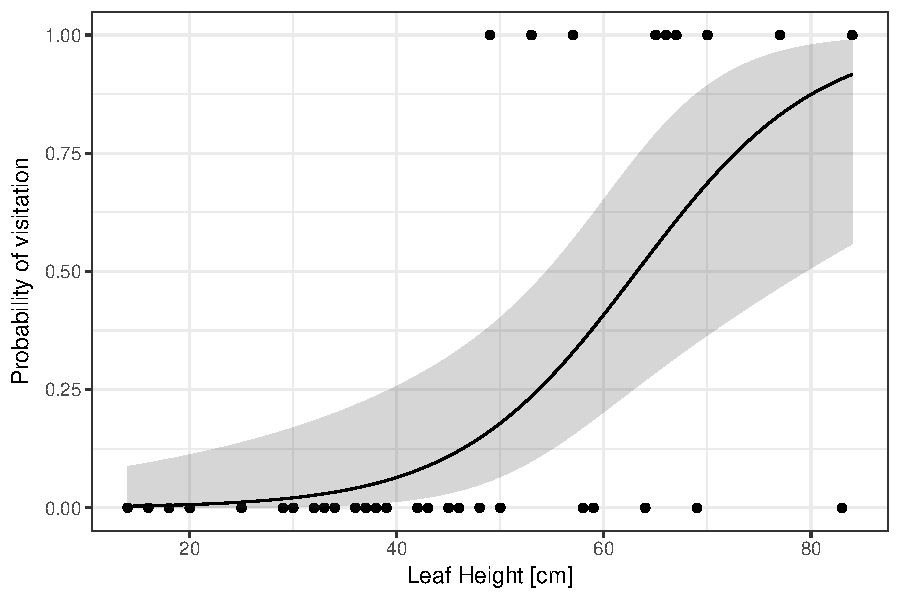
\includegraphics[width=0.7\linewidth]{01-glms_files/figure-beamer/plot-darlingtonia-1} \end{center}

\end{frame}

\begin{frame}{Wald statistics}

\(z\) values are Wald statistics, which under the null hypothesis follow
\emph{assymptotically} a standard normal distribution

Tests the null hypothesis that \(\beta_i = 0\)
\[z = \hat{\beta}_i / \mathrm{SE}(\hat{\beta}_i)\]

\begin{longtable}[]{@{}lrrrr@{}}
\toprule
& Estimate & Std. Error & z value &
Pr(\textgreater{}\textbar{}z\textbar{})\tabularnewline
\midrule
\endhead
(Intercept) & -7.2930 & 2.1608 & -3.3751 & 0.0007\tabularnewline
leafHeight & 0.1154 & 0.0365 & 3.1575 & 0.0016\tabularnewline
\bottomrule
\end{longtable}

\end{frame}

\begin{frame}{Deviance}

\begin{itemize}
\tightlist
\item
  In least squares we have the residual sum of squares as the measure of
  lack of fitted
\item
  In GLMs, \alert{deviance} plays the same role
\item
  Deviance is defined as twice the log likelihood of the observed data
  under the current model
\item
  Deviance is defined relative to an arbitrary constant --- only
  \alert{differences} of deviances have any meaning
\item
  Differences in deviances are also known as ratios of likelihoods
\item
  An alternative to the Wald tests are deviance ratio or likelihood
  ratio tests
  \[F = \frac{(D_a - D_b) / (\mathsf{df}_a - \mathsf{df}_b)}{D_b / \mathsf{df}_b}\]
\item
  \(D_j\) deviance of model, where we test if model A is a significant
  improvement over model B; \(\mathsf{df}_k\) are the degrees of freedom
  of the respective model
\end{itemize}

\end{frame}

\begin{frame}{A Gamma GLM --- simple age-depth modelling}

\begin{itemize}
\tightlist
\item
  Radiocarbon age estimates from depths within a peat bog (Brew \&
  Maddy, 1995, QRA Technical Guide No.\textasciitilde{}5)
\item
  Estimate accumulation rate; assumption here is linear accumulation
\item
  Uncertainty or error is greater at depth; mean variance relationship
\item
  Fit mid-depth \& mid-calibrated age points
\end{itemize}

\scriptsize

\begin{longtable}[]{@{}lrrrrrrrr@{}}
\toprule
Sample & upperDepth & lowerDepth & ageBP & ageError & calUpper &
calLower & midDepth & calMid\tabularnewline
\midrule
\endhead
SRR-4556 & 20 & 22.0 & 355 & 35 & 509 & 307 & 19.00 &
408.0\tabularnewline
SRR-4557 & 26 & 28.0 & 465 & 35 & 542 & 480 & 25.00 &
511.0\tabularnewline
SRR-4558 & 32 & 34.0 & 635 & 35 & 671 & 545 & 31.00 &
608.0\tabularnewline
SRR-4559 & 38 & 40.0 & 740 & 35 & 732 & 666 & 37.00 &
699.0\tabularnewline
SRR-4560 & 44 & 46.0 & 865 & 35 & 916 & 691 & 43.00 &
803.5\tabularnewline
SRR-4561 & 50 & 52.5 & 870 & 35 & 918 & 692 & 48.75 &
805.0\tabularnewline
SRR-4562 & 56 & 58.0 & 985 & 35 & 967 & 795 & 55.00 &
881.0\tabularnewline
SRR-4563 & 100 & 108.0 & 1270 & 35 & 1284 & 1097 & 96.00 &
1190.5\tabularnewline
SRR-4564 & 200 & 207.0 & 2575 & 35 & 2761 & 2558 & 196.50 &
2659.5\tabularnewline
SRR-4565 & 260 & 268.0 & 3370 & 35 & 3697 & 3487 & 256.00 &
3592.0\tabularnewline
SRR-4566 & 400 & 407.0 & 4675 & 35 & 5563 & 5306 & 396.50 &
5434.5\tabularnewline
SRR-4567 & 493 & 500.0 & 5315 & 35 & 6263 & 5955 & 489.50 &
6109.0\tabularnewline
\normalsize & & & & & & & &\tabularnewline
\bottomrule
\end{longtable}

\end{frame}

\begin{frame}{A Gamma GLM --- simple age-depth modelling}

\begin{center}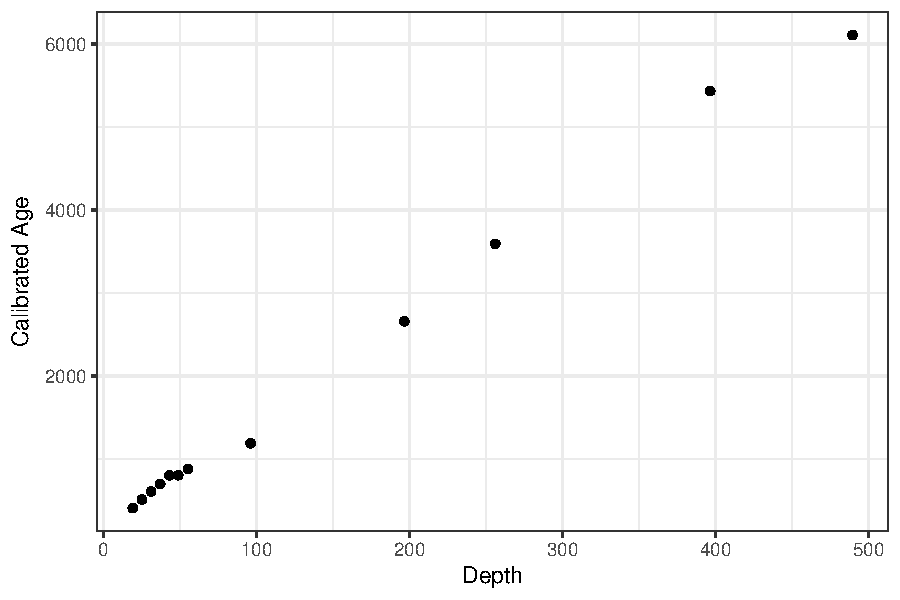
\includegraphics[width=0.7\linewidth]{01-glms_files/figure-beamer/plot-maddy-1} \end{center}

\end{frame}

\begin{frame}[fragile]{A Gamma GLM --- simple age-depth modelling}

\begin{Shaded}
\begin{Highlighting}[]
\NormalTok{>}\StringTok{ }\NormalTok{mod <-}\StringTok{ }\KeywordTok{glm}\NormalTok{(calMid ~}\StringTok{ }\NormalTok{midDepth, }\DataTypeTok{data =} \NormalTok{maddy, }\DataTypeTok{family =} \KeywordTok{Gamma}\NormalTok{(}\DataTypeTok{link =} \StringTok{"identity"}\NormalTok{))}
\NormalTok{>}\StringTok{ }\KeywordTok{summary}\NormalTok{(mod)}
\end{Highlighting}
\end{Shaded}

\begin{verbatim}

Call:
glm(formula = calMid ~ midDepth, family = Gamma(link = "identity"), 
    data = maddy)

Deviance Residuals: 
      Min         1Q     Median         3Q        Max  
-0.161184  -0.016734  -0.002595   0.048033   0.085943  

Coefficients:
            Estimate Std. Error t value Pr(>|t|)    
(Intercept) 197.2909    22.5603   8.745 5.35e-06 ***
midDepth     12.5799     0.4543  27.693 8.74e-11 ***
---
Signif. codes:  0 '***' 0.001 '**' 0.01 '*' 0.05 '.' 0.1 ' ' 1

(Dispersion parameter for Gamma family taken to be 0.004612561)

    Null deviance: 10.439047  on 11  degrees of freedom
Residual deviance:  0.048316  on 10  degrees of freedom
AIC: 145.57

Number of Fisher Scoring iterations: 4
\end{verbatim}

\end{frame}

\begin{frame}{A Gamma GLM --- simple age-depth modelling}

\begin{center}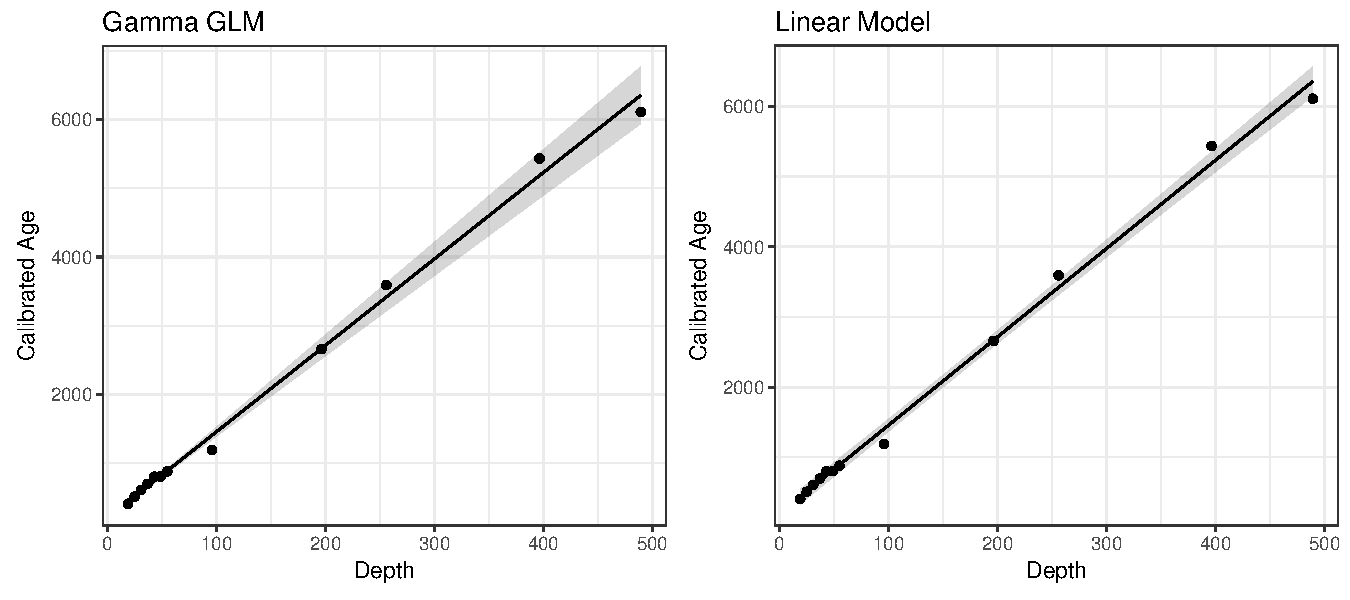
\includegraphics[width=0.9\linewidth]{01-glms_files/figure-beamer/plot-maddy-fitted-1} \end{center}

\end{frame}

\begin{frame}{Re-use}

Copyright © (2017) Gavin L. Simpson Some Rights Reserved

Unless indicated otherwise, this slide deck is licensed under a
\href{http://creativecommons.org/licenses/by/4.0/}{Creative Commons
Attribution 4.0 International License}.

\begin{center}
  \ccby
\end{center}

\end{frame}

\end{document}
